%---------------------------------------------------------------------------
% Knowledge component.
%
%---------------------------------------------------------------------------
\section{Knowledge component}
\label{sec:arch_knowledge}

The Knowledge component is responsible for the realization of a semantic-based approach to the proposed system. Although the end-user can barely notice its existence, it is crucial to allow a high scalability and an ease of use. The ontologies built-in to the system provide the generic measurement semantics. Such an approach allows the user to get to know the system only once and work using it with many different types of hardware, protocols. The user is enabled to work with any measurable item type that can be mapped into a generic component introduced by the ontology. Additionally it allows to work with all those different items simultaneously; thus, it makes it possible to monitor an application that is written using different, cooperating technologies.

\subsection{Default ontologies}

All system functionalities are built around two main ontologies - the first one grouping resources, and the second, covering resource capabilities. The main principle, I was trying to follow when designing them was to expand the types of applications that can be monitored using the SemSimMon system - from these running a single process on one computer, up to highly distributed, grid-oriented ones.

Two root concepts are going to be explained: the concept of resource and of capability, in order to describe the proposed ontologies in more details. The resource class wraps all components that are used to perform required computations. Resource can be a physical device that takes part in a computation (hardware resources), or any software component that is either a dependency (library) or something that the user creates (program, library). The capability concept generalizes all tje measurable features of each resource. Capabilities exist only in the context of a resource that contain them. Resource may have multiple capabilities and a given capability may exist within the context of multiple resources.

Both these ontologies are described using diagrams, containing two types of relationships: \lq\lq{}\emph{is-a}\rq\rq{}, and \lq\lq{}\emph{has-a}\rq\rq{}. The \lq\lq{}\emph{is-a}\rq\rq{} relationship is formalized as \texttt{rdfs:subClassOf} and states that all instances of one class are instances of another~\cite{rdfRef:2004}. The \lq\lq{}\emph{has-a}\rq\rq{} relationship describes resources only. The main purpose of this relationship is to show the composition arrangement. It aims at easing understanding of which resources a given parent resource use (e.g. virtual machine uses class loader, garbage collector; one or more CPUs builds a computing node, storage device, network device, and so on).

In the diagrams that follow, entities are drawn as a filled ellipse with an entity name inside. The graphical representation of the \lq\lq{}\emph{is-a}\rq\rq{} relationship between two entities is a hollow triangle shape on the super type end of the line that connects it to one or more subtypes. Diagrams use a line with an arrowhead indicating an owned side of a relationship to represent the \lq\lq{}\emph{has-a}\rq\rq{} relation. A UML use case diagram specification was the source of an inspiration for this notation.

\subsection{Resources ontology}
\label{subsec:arch_knowledge_resources}

The complexity of the resources ontology forced the author to split diagrams containing both \lq\lq{}\emph{is-a}\rq\rq{} and \lq\lq{}\emph{has-a}\rq\rq{} relationships into 3 parts: the one containing the most general classes (application, node, and cluster), the second one for hardware resources and the third one, covering the software resources. 

\begin{figure}[ht]
\centering
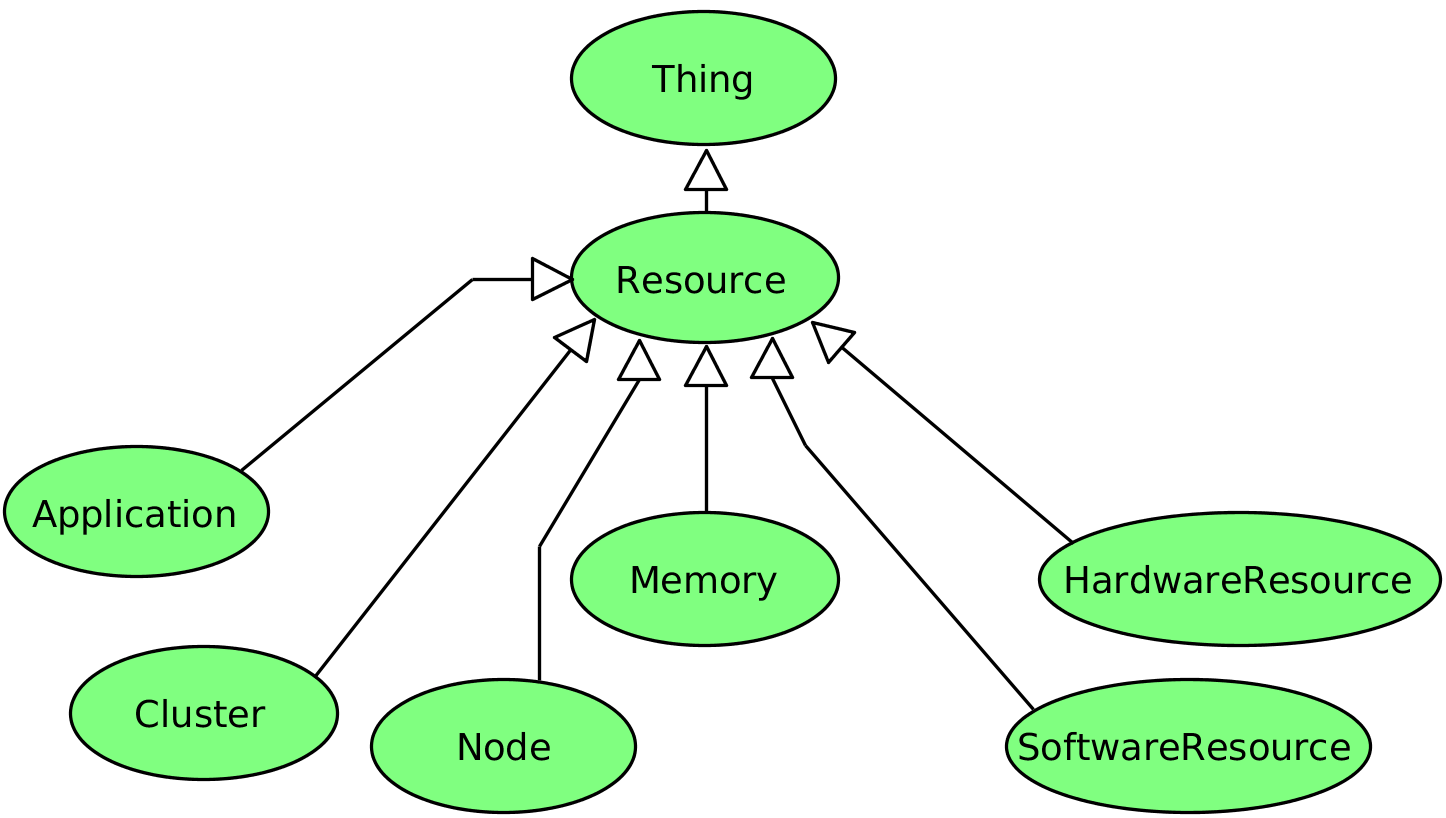
\includegraphics[width=0.6\textwidth]{onto_resources_admin}
\caption{Diagram of the \lq\lq{}\emph{is-a}\rq\rq{} (\texttt{rdfs:subClassOf}) relationship between the most general resource concepts}
\label{fig:onto_resources_admin}
\end{figure}

Figure~\ref{fig:onto_resources_admin} depicts the \lq\lq{}\emph{is-a}\rq\rq{} relationship between general SemSimMon\rq{}s concepts. The root class of each entity in OWL compliant ontologies is the \texttt{owl:Thing}, as specified in OWL language reference~\cite{owlRef:2009}. I have introduced a generic \texttt{Resource} class to cover all possible resources. It acts as a root concept for all other resources and the only one that is a direct subclass of the \texttt{owl:Thing}. The \texttt{Resource} has 6 direct subtypes: \texttt{Application}, \texttt{Cluster}, \texttt{Node}, \texttt{Memory}, \texttt{HardwareResource} and \texttt{SoftwareResource}. The \texttt{Application} and \texttt{Cluster} types are so called \lq\lq{}management\rq\rq{} class resources - they do not represent actual components, which can be used to perform computations. Instead, they can be used to group one or more elements, that allows the user to build more manageable measurement structures. The \texttt{Application} is the most notable entity type, in the context of the \lq\lq{}\emph{has-a}\rq\rq{} relationship, which is illustrated in Figure~\ref{fig:onto_resources_has_a_admin}. It represents a program created by the user that he or she wants to analyze using the proposed tool. Each application, in a theoretical model may be running on multiple clusters, and multiple nodes.

The \texttt{Cluster} refers to a group of computing nodes, which are connected using a high-efficiency network; thus, in some way it may be treated as a single entity. It is equivalent of a \lq\lq{}site\rq\rq{} in the OMIS nomenclature~\cite{tl9702e}. The \texttt{Node} class can be interpreted as a bridge between high-level resources and software, hardware resources. It is the smallest independent computing unit, e.g. a single PC or a unit in a rack. It can be treated as an administrative resource type, as it is not a component that is used directly, but one that uses these components. On the other hand, a node is an actual processing device.

There exist also a noteworthy class of resources - the \texttt{Memory}. There are at least two types of memory: a software based (virtual memory) and a hardware (physical memory) that share common semantics which can be easily described within this type.

\begin{figure}[ht]
\centering
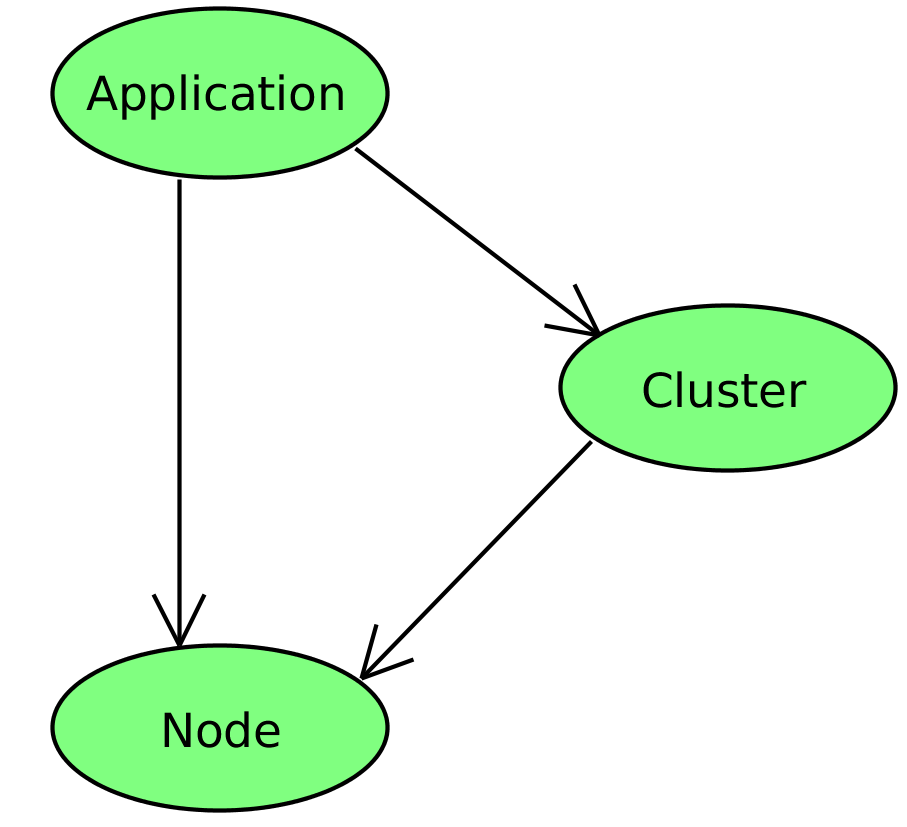
\includegraphics[width=0.3\textwidth]{onto_resources_has_a_admin}
\caption{Diagram of the \lq\lq{}\emph{has-a}\rq\rq{} relationship between the most general resource concepts}
\label{fig:onto_resources_has_a_admin}
\end{figure}

\begin{figure}[ht]
\centering
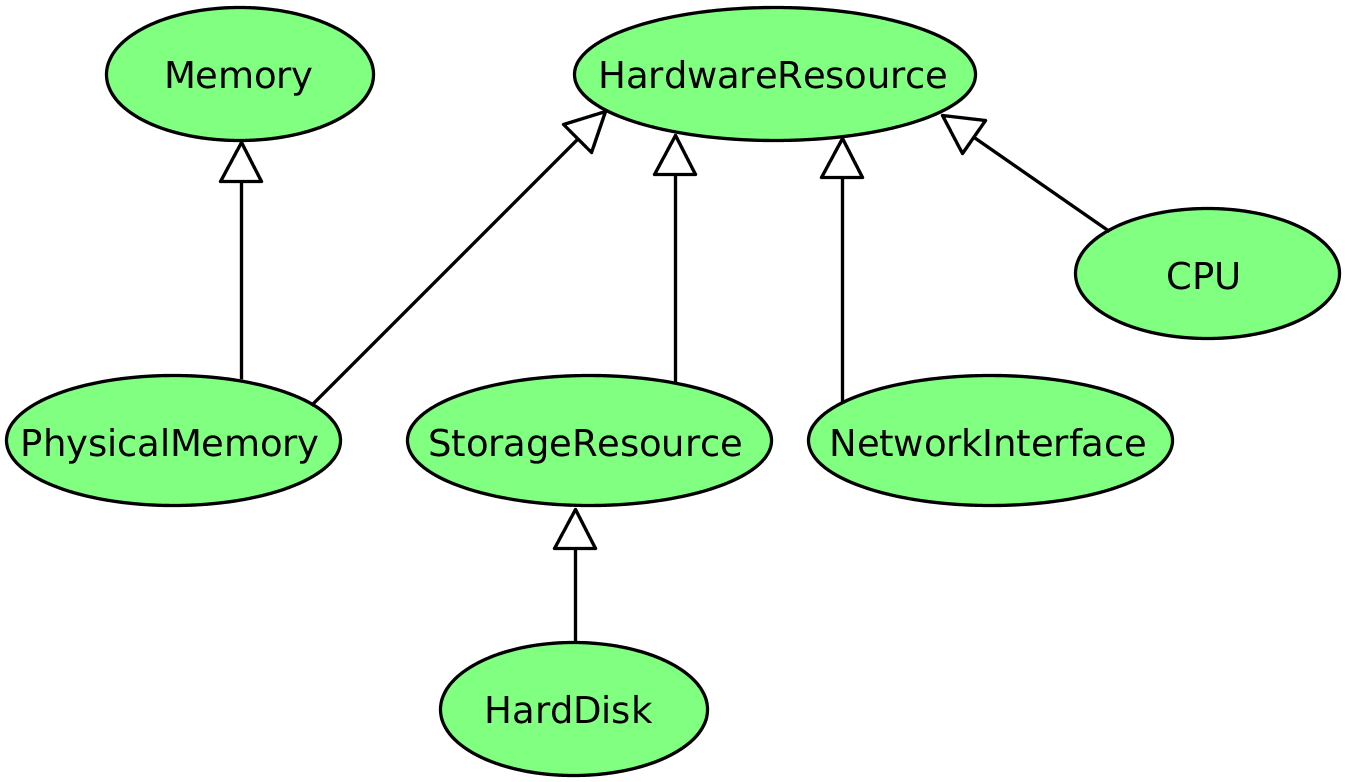
\includegraphics[width=0.6\textwidth]{onto_resources_hardware}
\caption{Diagram of the \lq\lq{}\emph{is-a}\rq\rq{} relationship between hardware resources}
\label{fig:onto_resources_hardware}
\end{figure}

The classes related to hardware resources, can be seen in Figures~\ref{fig:onto_resources_hardware} and~\ref{fig:onto_resources_has_a_hardware}. The design of all of them allows covering most of computer parts available nowadays on the market. Both diagrams are quite straightforward. The \texttt{HardwareResource} has 4 direct sub-types: \texttt{PhysicalMemory}, \texttt{StorageResource}, \texttt{NetworkInterface} and \texttt{CPU}. The \texttt{PhysicalMemory}, is also a subtype of the \texttt{Memory} class, to share common semantics. Also, the \texttt{StorageResource} has one derived class - \texttt{HardDisk}. The hardware resources\rq{} \lq\lq{}\emph{has-a}\rq\rq{} relationship diagram is even more elementary - the \texttt{Node} may have all hardware resources, and there are no other relations between those resources.

\begin{figure}[ht]
\centering
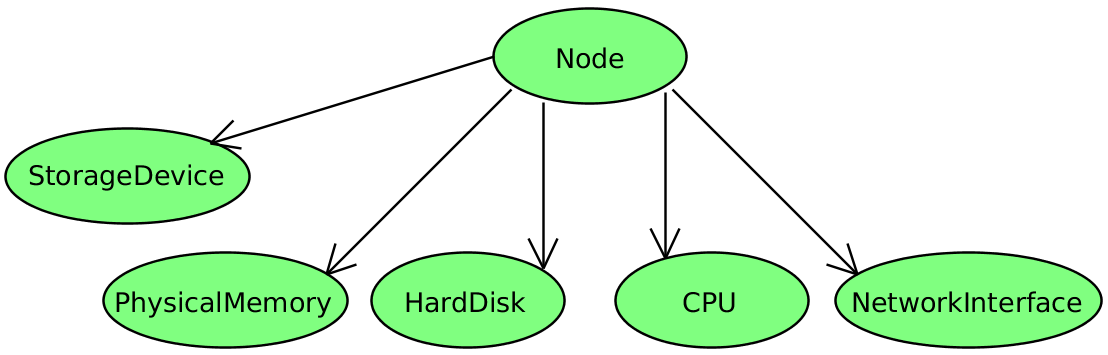
\includegraphics[width=0.7\textwidth]{onto_resources_has_a_hardware}
\caption{Diagram of the \lq\lq{}\emph{has-a}\rq\rq{} relationship between hardware resources}
\label{fig:onto_resources_has_a_hardware}
\end{figure}

\begin{figure}[ht]
\centering
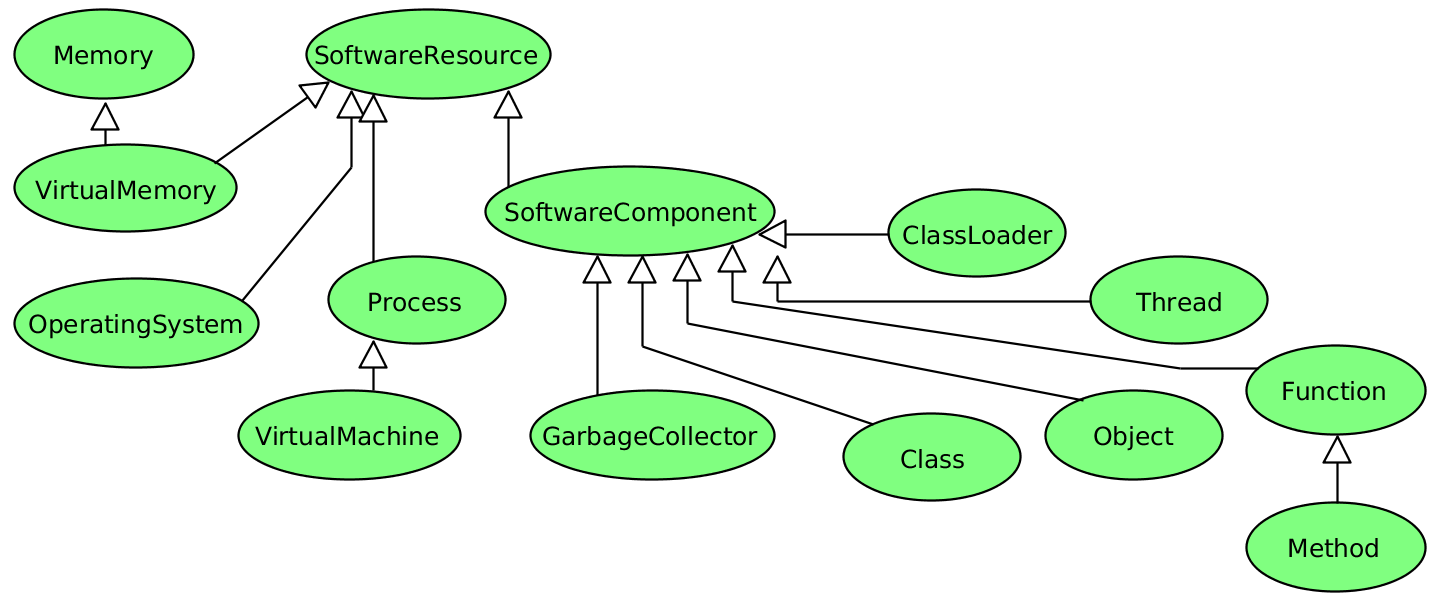
\includegraphics[width=0.9\textwidth]{onto_resources_software}
\caption{Diagram of the \lq\lq{}\emph{is-a}\rq\rq{} relationship between software resources}
\label{fig:onto_resources_software}
\end{figure}

The system is aware of software resource types to a greater extent then hardware ones. This implies sophisticated relationships between concepts depicted in Figures~\ref{fig:onto_resources_software} and~\ref{fig:onto_resources_has_a_software}. The \texttt{SoftwareResource} class has 4 direct subtypes: \texttt{VirtualMemory} (which also derives from the generic \texttt{Memory} concept), \texttt{OperatingSystem}, \texttt{Process} and \texttt{SoftwareComponent} concept. The first three types are quite straightforward and represent what one expects them to do. A special subtype of the \texttt{Process}, namely the \texttt{VirtualMachine} needs a more concern. It was extracted from a general type, due to its nature, which distinguishes it from all general-purpose processes. Each virtual machine acts as a runtime environment for running applications; thus, it has features common for all virtual machines, but unlikely seen in plain processes. The \texttt{SoftwareComponent} resource type is a logical wrapper for all low-level software components that can be used to create a program. There are generic components, like \texttt{Thread}, \texttt{Function}. There are also types specific to Object Oriented Programming: \texttt{Class}, \texttt{Object}, and \texttt{Method} (which subtypes \texttt{Function}). The third group of \texttt{SoftwareComponent} subtypes is specific to virtual machines. It contains only two items: \texttt{GarbageCollector} and \texttt{ClassLoader}.

Regarding the ownership relations in the software category, there is one root concept - the \texttt{Node}. Each node has an \texttt{OperatingSystem}, and multiple \texttt{Processes}. Some processes may be a \texttt{VirtualMachine}, which makes this resource the last type that the \texttt{Node} may directly own. Each \texttt{Process} may have the following software components: \texttt{Thread}, \texttt{Object}, \texttt{Class} and \texttt{Function}. The \texttt{VirtualMachine} may have all the components that the generic \texttt{Process} has and two more specific ones: \texttt{ClassLoader} and \texttt{GarbageCollector}. Additionally, the \texttt{Class} type owns a single resource type, the \texttt{Method}. The \texttt{OperatingSystem} resource may have only one software resource type, namely a \texttt{VirtualMemory}.

\begin{figure}[ht]
\centering
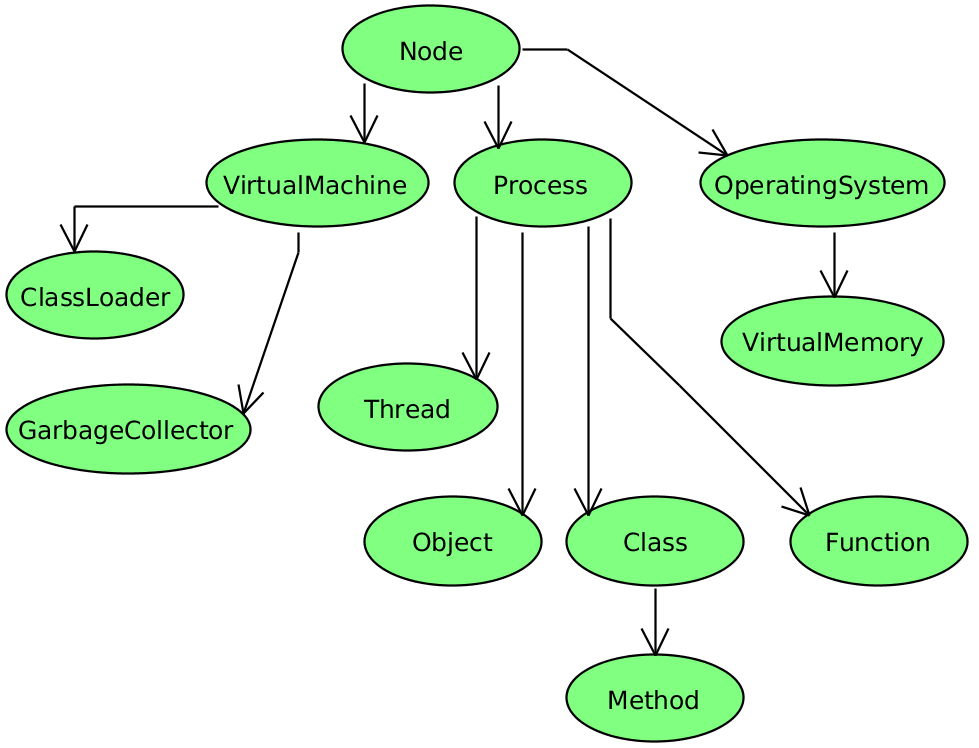
\includegraphics[width=0.7\textwidth]{onto_resources_has_a_software}
\caption{Diagram of the \lq\lq{}\emph{has-a}\rq\rq{} relationship between software resources}
\label{fig:onto_resources_has_a_software}
\end{figure}

\pagebreak

\subsection{Capabilities ontology}
\label{subsec:arch_knowledge_capabilitie}

For the concepts related to the capabilities of resources, only the \lq\lq{}\emph{is-a}\rq\rq{} relationship was defined, which is illustrated in Figure~\ref{fig:onto_capabilities}. There is one root concept, namely \texttt{ResourceCapability}, which subclasses \texttt{rdf:Thing}. It has 4 direct subtypes: \texttt{HardwareCapability}, \texttt{MemoryCapability}, \texttt{NodeCapability} and \texttt{SoftwareCapability}. \texttt{HardwareCapability} has only 2 derived classes: \texttt{StorageCapability} and \texttt{CpuCapability}. Since the concepts of \texttt{VirtualMemory} and \texttt{PhysicalMemory} are semantically close, there is no need to subclass generic \texttt{MemoryCapability}; thus, this type does not have any subtypes. The \texttt{NodeCapability} is another direct subtype of the most generic \texttt{ResourceCapability}, which does not require any additional child types.

The complex structure of software resources influences the relationships between the capabilities related to those components. The \texttt{SoftwareCapability} has 3 subtypes: \texttt{OperatingSystemCapability}, \texttt{ProcessCapability} and \texttt{SoftwareComponentCapability}. Additionally, \texttt{VirtualMachineCapability} was extracted from \texttt{ProcessCapability}, because of the same reasons that motivate the extraction of the \texttt{VirtualMachine} resource type from the \texttt{Process} - different semantics. The single type that extends the \texttt{SoftwareComponentCapability} is the \texttt{ThreadCapability}.

\begin{figure}[ht]
\centering
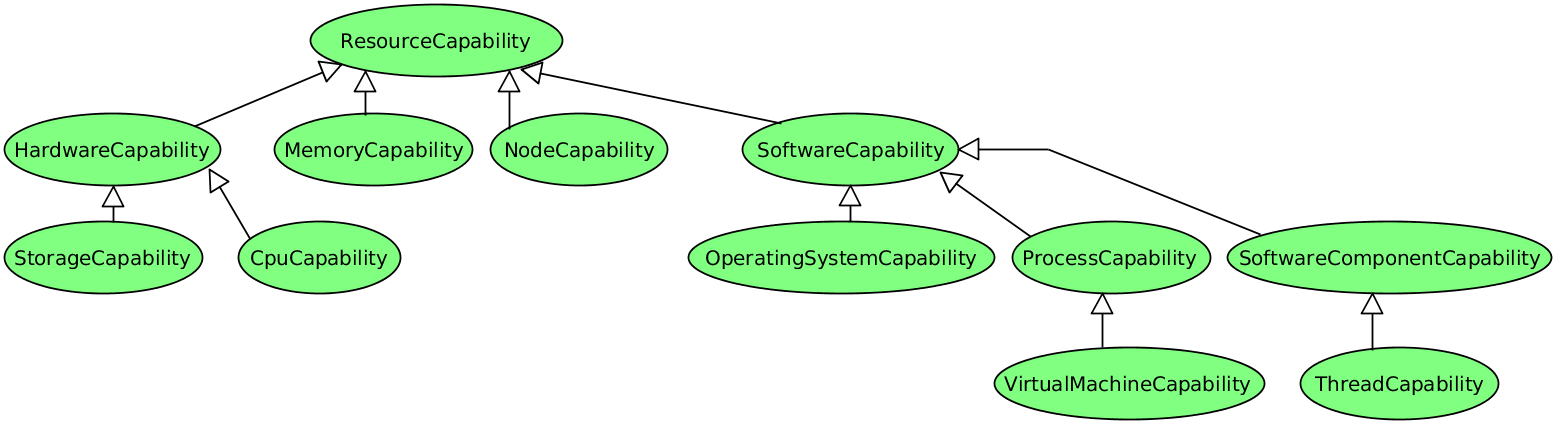
\includegraphics[width=1.0\textwidth]{onto_capabilities}
\caption{Diagram of the \lq\lq{}\emph{is-a}\rq\rq{} relationship between capabilities}
\label{fig:onto_capabilities}
\end{figure}

